
\subsection{Background}
    The first paradigm used to solve the VLSI optimization problem is Constraint Programming (CP),
    developed using MiniZinc as modeling language. 
    Starting from a base model following the constraints discussed in \ref{sec:shared_constraints},
    we added: rotation variables \ref{eq:rotation_vars}, symmetry breaking constraints and search strategies;
    to be more precise we have a model for each combination of the previous elements.
    To test different behaviour of solvers we have chosen to run each model on both Chuffed and Gecode solvers.

    \colorbox{BurntOrange}{TODO missing ...}

% % % % % % % % % % % % % % % % % % % % % % % % % % % % % % % % % % % % % % % % % % % % % % % % % %

\subsection{Variables}
    In CP we tried to break also the symmetries due to \textit{virtual} circuits, but, as already
    explained in section \ref{sec:symmetries}, we decided to keep only the simplest ones that will 
    be described soon.

    This section is mainly needed to introduce variables related to \textit{virtual} circuits
    
    \begin{align}
        vc_{i,j}    &\ =\ \text{\textit{virtual} circuit obtained from  } (i,j) \in CC  \\
        n\_vc\      &\ =\ \text{maximum number of \textit{virtual} circuits}            \\
        n\_rvc\     &\ =\ n\_vc + nc                                                    \\
        VC          &\ =\ \{ c_i\ |\ i \in [1,n\_vc] \}                                 \\
        RVC         &\ =\ \{ c_i\ |\ i \in [1,n\_rvc] \}                                \\
        % c_pairs &\ =\ [(i,j)\ |\ (i,j) \in CC]
    \end{align}

    The first definition needs deeper explanation: a rectangle can be defined giving the position
    of its bottom left and its top right corner and for a \textit{virtual} circuit they are the
    bottom left corner of circuit $i$ and the top right corner of circuit $j$.
    

% % % % % % % % % % % % % % % % % % % % % % % % % % % % % % % % % % % % % % % % % % % % % % % % % %

\subsection{Predicates \& Functions}
    The additional predicates and functions we define in this section will later be used in the models
    adopting symmetry breaking constraints and the ones allowing rotation of circuits, the others work 
    with the constraints already defined.

    \begin{align}
        vc\_x(vc_{i,j})\                        \leftarrow\ & min(x_i, x_j)                                 \\
        vc\_y(vc_{i,j})\                        \leftarrow\ & min(y_i, y_j)                                 \\
        vc\_width(vc_{i,j})\                    \leftarrow\ & max(x_i + w_i, x_j + w_j) - vc\_x(vc_{i,j})   \\
        vc\_height(vc_{i,j})\                   \leftarrow\ & max(y_i + h_i, y_j + h_j) - vc\_y(vc_{i,j})   \\
        vs\_is\_valid(vc_x, vc_y, vc_w, vc_h)   \leftarrow\ & \forall c \in C                               \\
                                                            & (\neg(x_c < vc_x \land x_c + w_c > vc_x) \land
                                                               \neg(x_c + w_c > vc_x + vc_w)) \nonumber     \\
                                                            &\ \hspace{4.7cm} \lor \nonumber                \\
                                                            & (\neg(y_c < vc_y \land y_c + h_c > vc_y) \land
                                                               \neg(y_c + h_c > vc_y + vc_h)) \nonumber
    \end{align}


    % \begin{align*}
    %     index\_set(X)\ &\ =\ \{i \in \mathbb{N}\ |\ 1 \leq i \leq |X|\}
    % \end{align*}

% % % % % % % % % % % % % % % % % % % % % % % % % % % % % % % % % % % % % % % % % % % % % % % % % %

\subsection{Constraints}
    \subsubsection{Base}
        The reference model is the one with the constraints described in section \ref{sec:symmetries}
        with the following simple symmetry breaking constraint:
        \begin{equation}
            x_1 <= x_2 \land y_1 <= y_2
        \end{equation}
        This constraint becomes meaningful since the circuits are first sorted according to their area.
    \colorbox{BurntOrange}{TODO missing ...}

    \begin{align*}
        Xcross(x)\ &\ =\ \{ c \in C\ |\ (x_c \leq x) \land (x_c + w_c > x) \} \\
        Ycross(y)\ &\ =\ \{ c \in C\ |\ (y_c \leq y) \land (y_c + h_c > y) \} 
    \end{align*}

    \begin{align}
        (x_i + w_i \leq x_j) \lor (y_i + h_i \leq y_j) &\ \ &\ \nonumber \\
        \lor\ (x_j + w_j \leq x_i) \lor (y_j + h_j \leq y_i)\ &\                \hspace{0.2cm} \forall (i,j) \in CC &\ \text{;diffn} \\
                                                                        \sum_{c \in C_x} y_c \leq makespan\ &\ \hspace{0.2cm} \forall x \in X, \forall c \in Xcross(x)\ &\ \text{;x axis} \\
                                                                           \sum_{c \in C_y} x_c \leq width\ &\ \hspace{0.2cm} \forall y \in Y, \forall c \in Ycross(y)\ &\ \text{;y axis}
    \end{align}

% % % % % % % % % % % % % % % % % % % % % % % % % % % % % % % % % % % % % % % % % % % % % % % % % %

\subsection{Rotation}
    \colorbox{BurntOrange}{TODO missing ...}

% % % % % % % % % % % % % % % % % % % % % % % % % % % % % % % % % % % % % % % % % % % % % % % % % %

\subsection{Search}
    \colorbox{BurntOrange}{TODO missing ...}

% % % % % % % % % % % % % % % % % % % % % % % % % % % % % % % % % % % % % % % % % % % % % % % % % %

\subsection{Results}
    \colorbox{BurntOrange}{TODO missing ...}

    % \begin{equation}
    %     \forall\ (i,j) \in A 
    %     \ \rightarrow \ 
    %     (x_i + w_i \leq x_j) \lor (y_i + h_i \leq y_j) \lor (x_j + w_j \leq x_i) \lor (y_j + h_j \leq y_i)
    %     \\
    %     \text{where:}\\
    %     A = { (i, j) | \, i \in index\_set(x), \, j \in index\_set(x), \, i<j }
    % \end{equation}

    \begin{figure}[H]
        \centering
        \begin{subfigure}[b]{1.0\textwidth}
            \centering 
            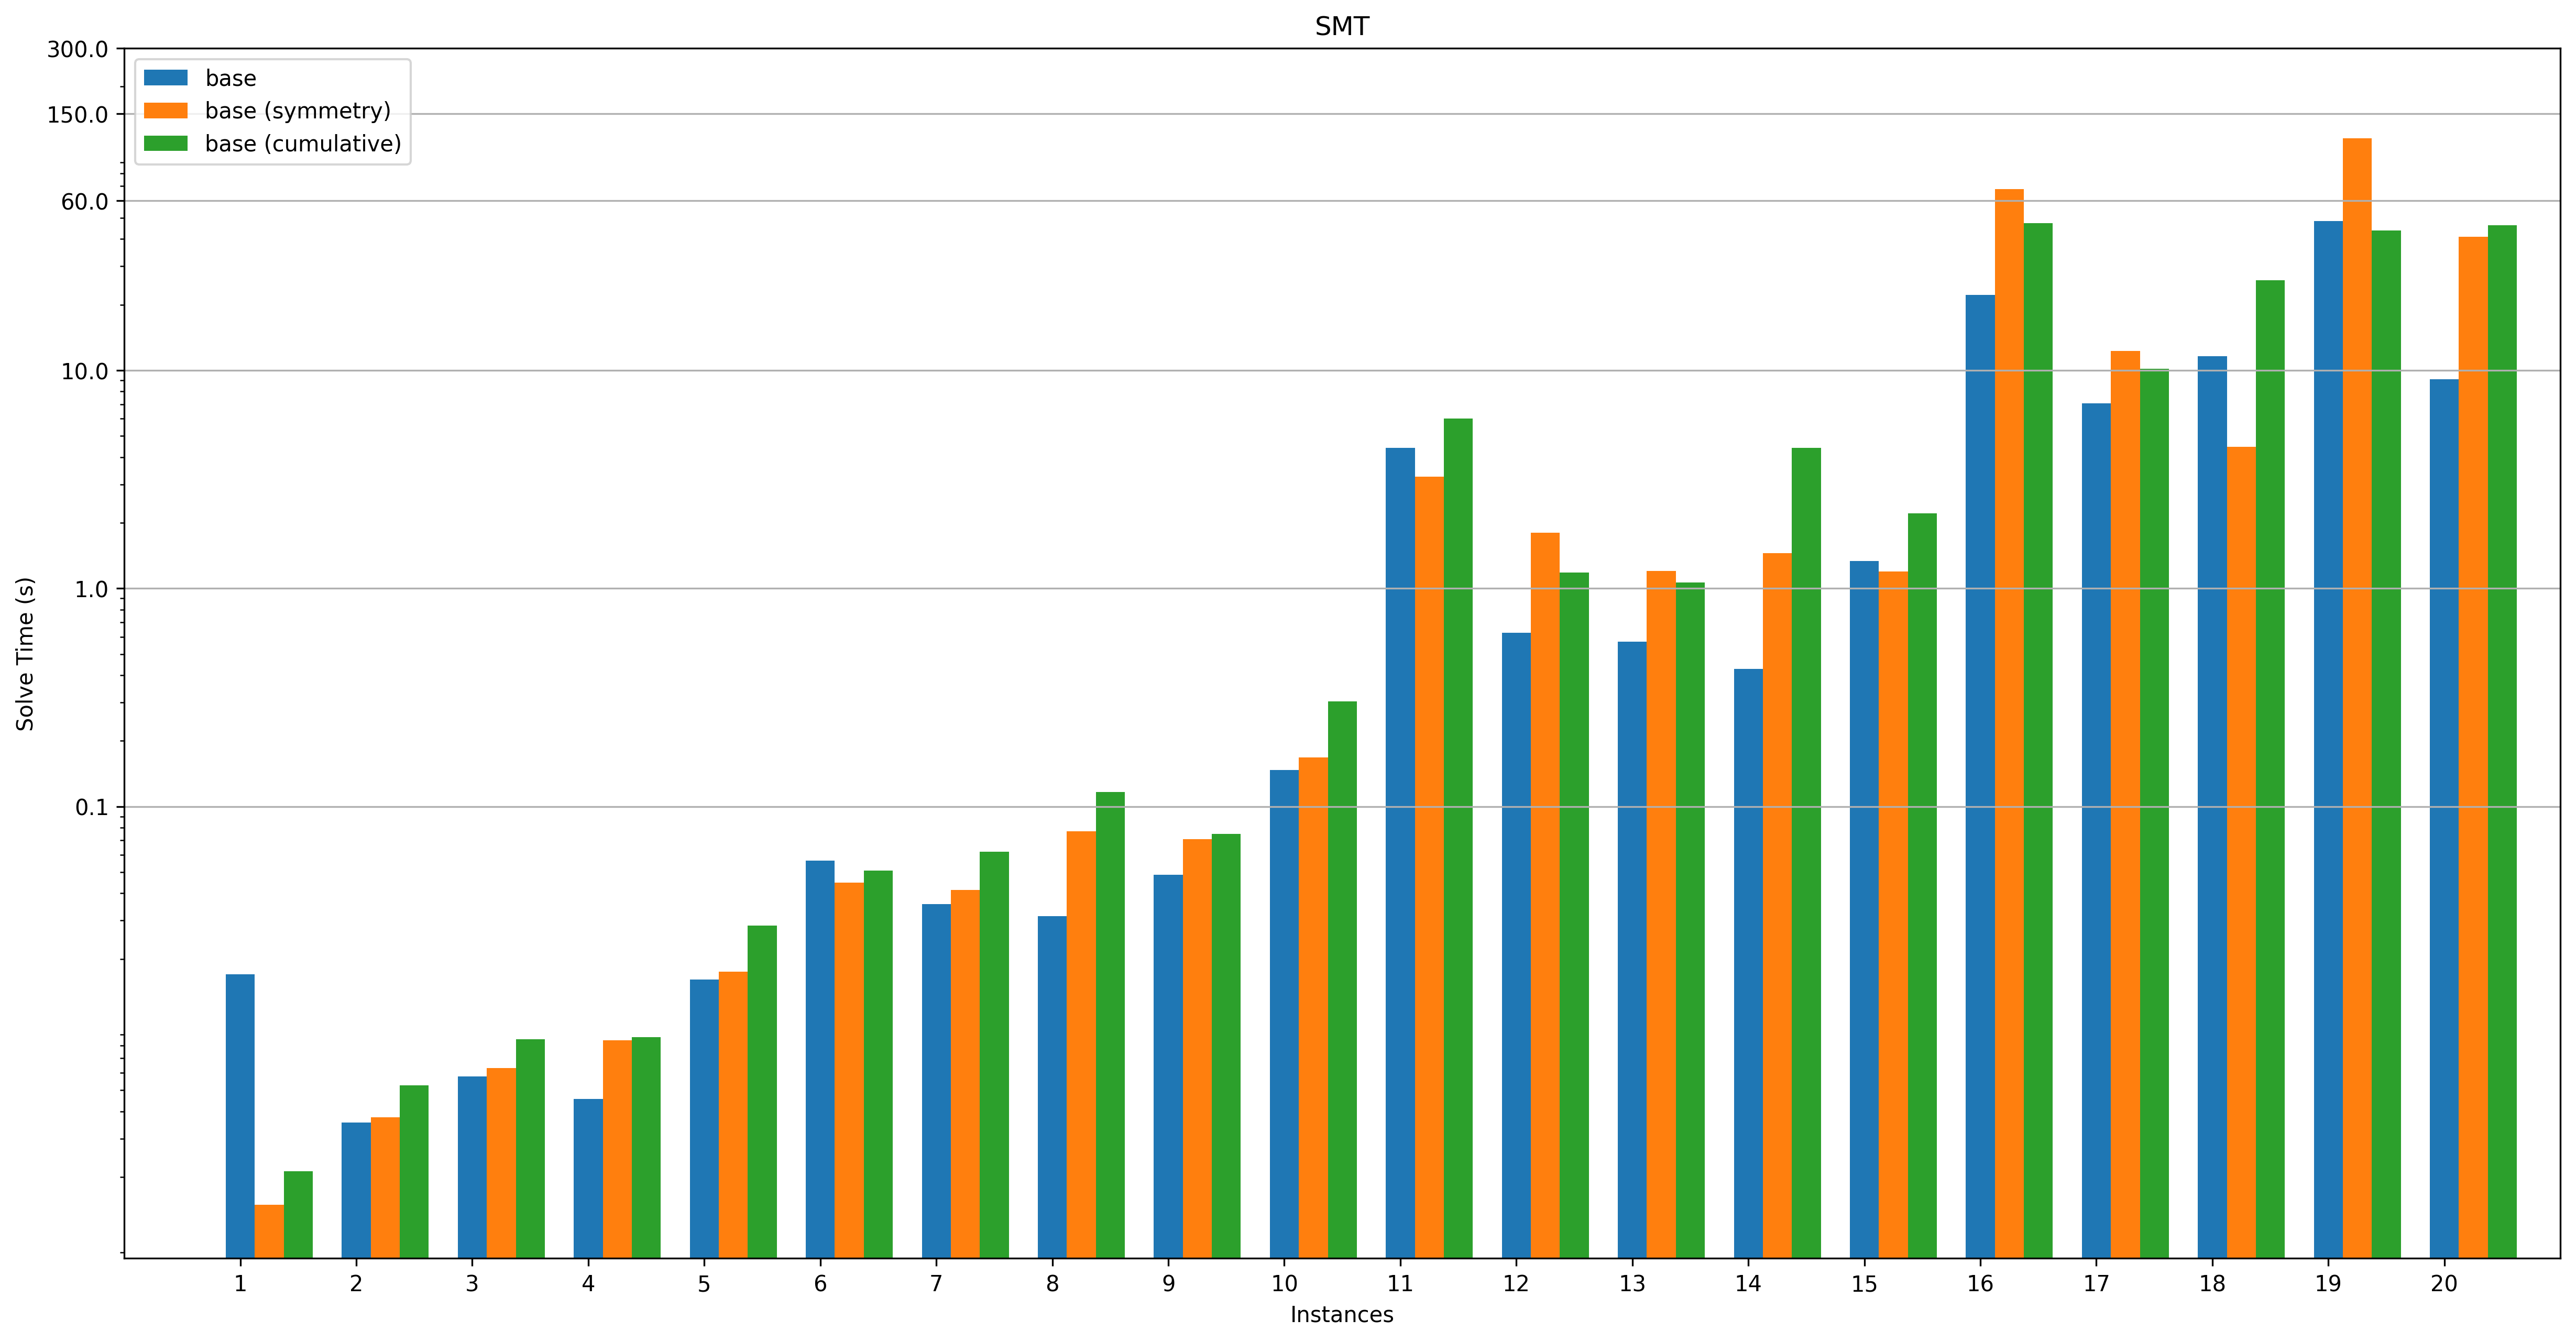
\includegraphics[width=\textwidth]{02/results_1.png}
            \caption{}
            \label{fig:vgpijerbgvpiberq}
        \end{subfigure}
        \begin{subfigure}[b]{1.0\textwidth}
            \centering
            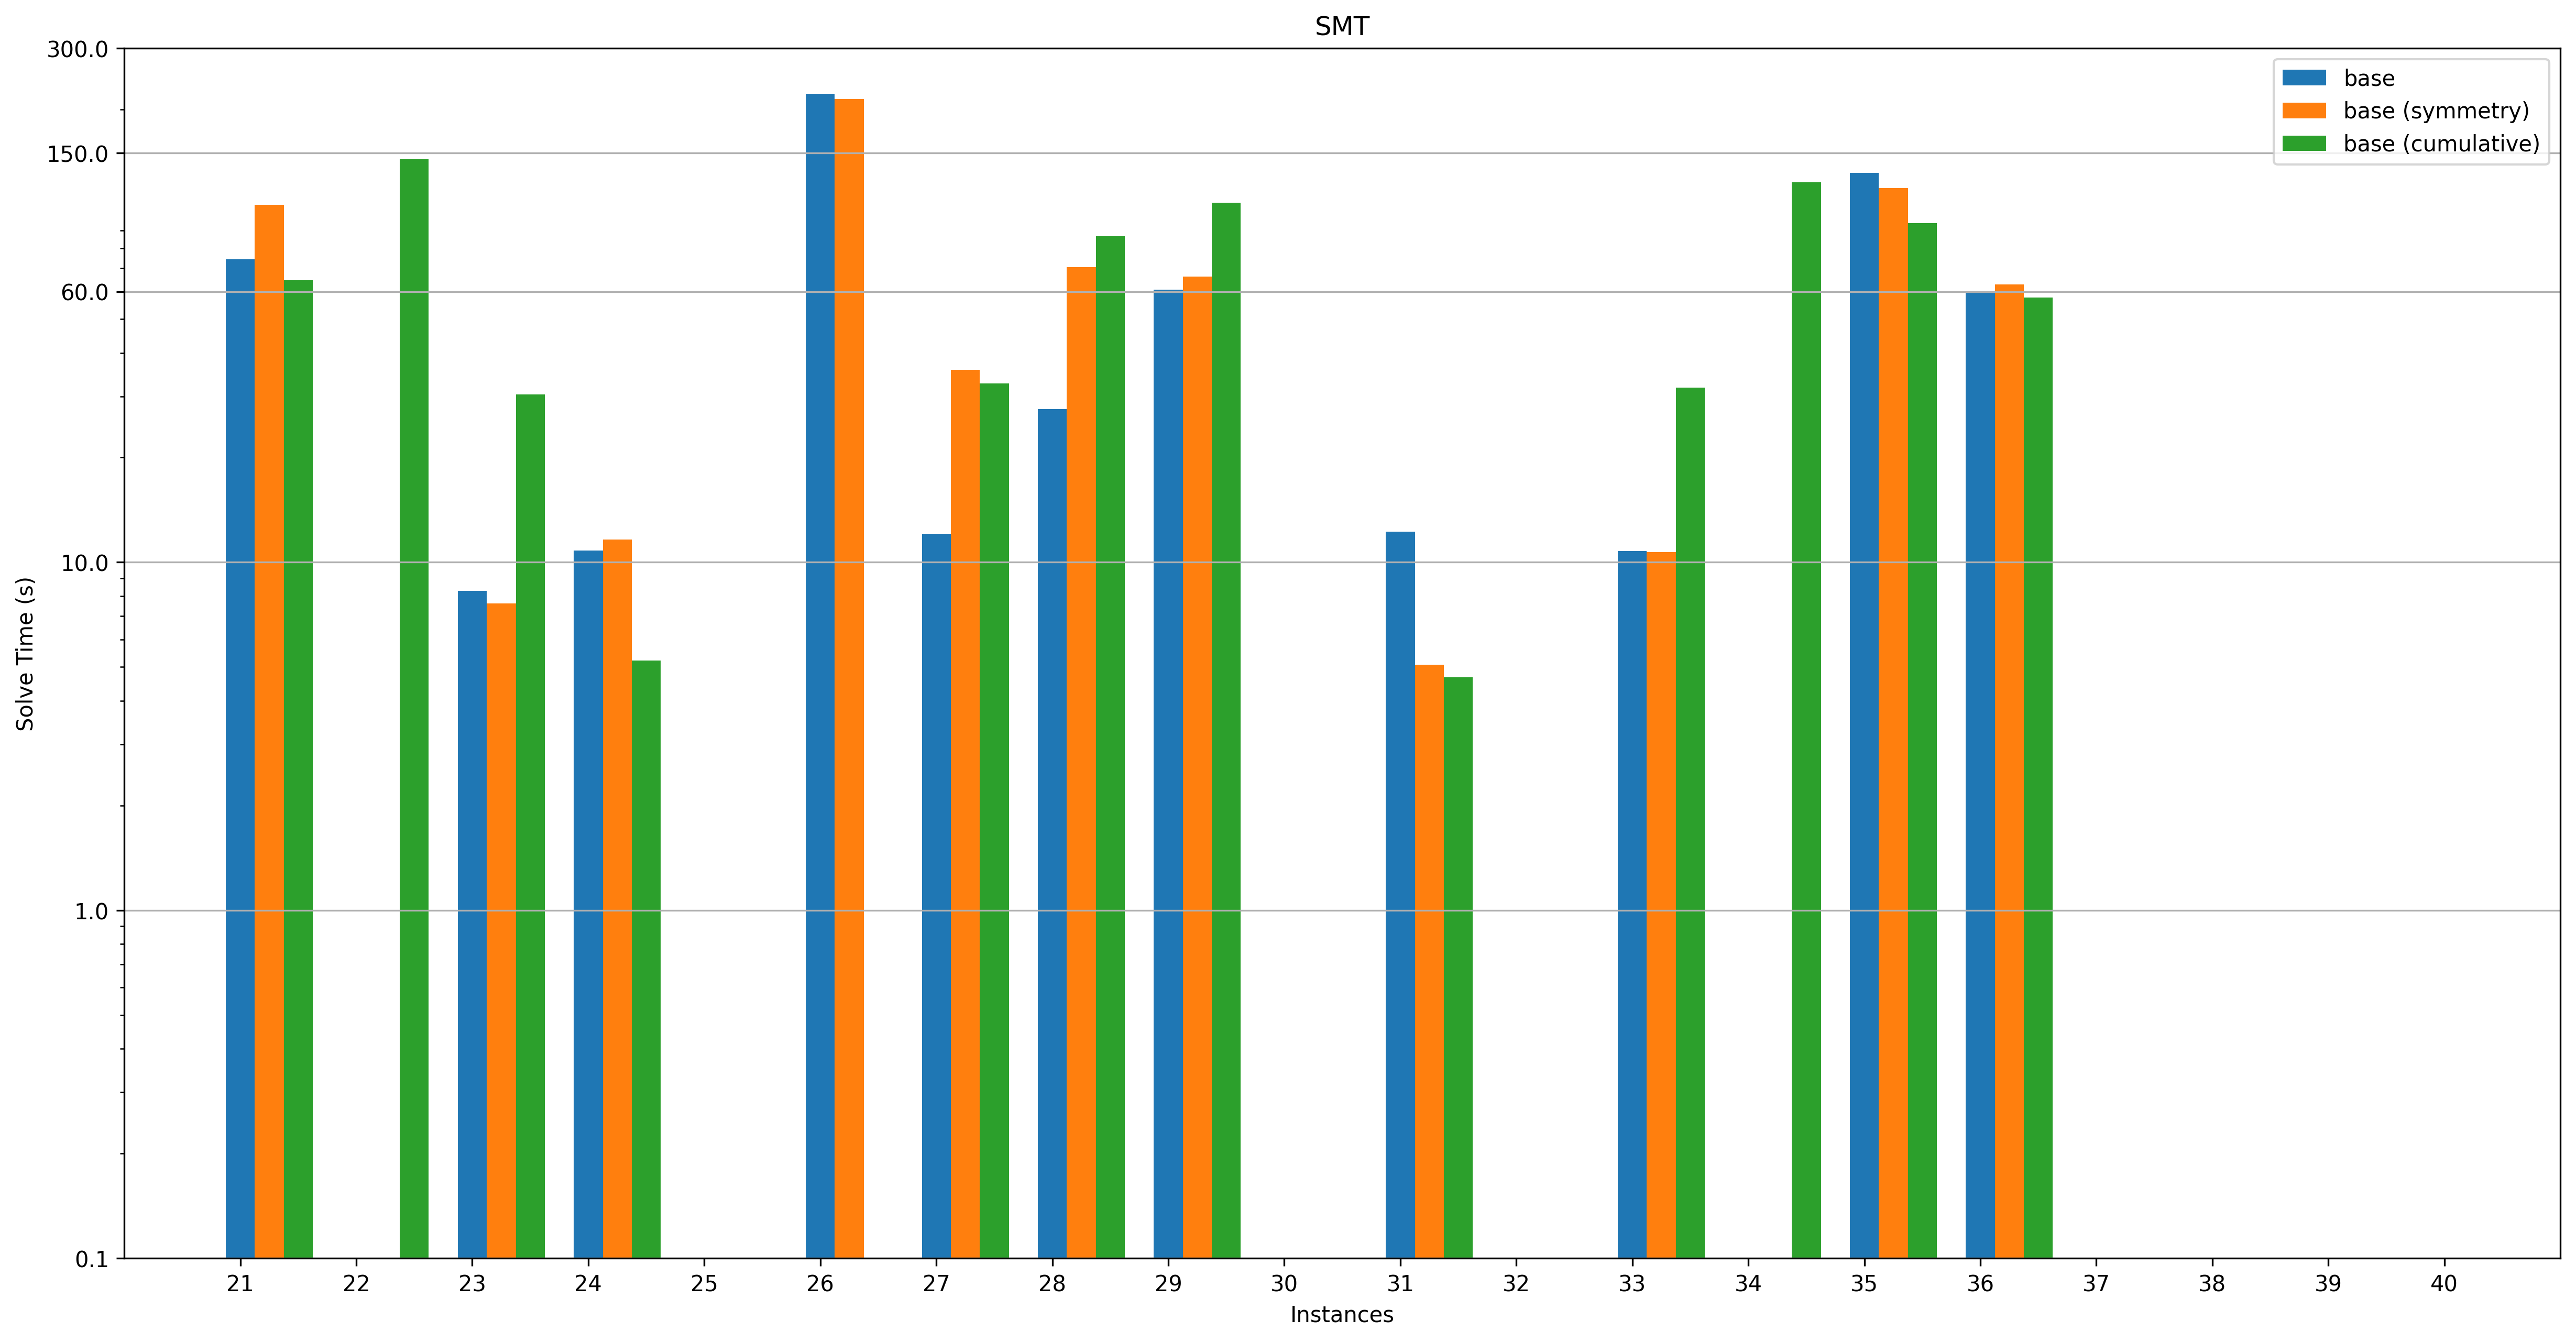
\includegraphics[width=\textwidth]{02/results_2.png}
            \caption{}
            \label{fig:vjidqenvjqen}
        \end{subfigure}
        \caption{weeeeeeeeeeee}
        \label{fig:vneqpwijvnpjewqnpivnenq}
    \end{figure}

\subsection{Virtual Circuits}
    \colorbox{BurntOrange}{TODO missing ...}
